\documentclass[aspectratio=169,11pt]{beamer}

\def\courseTitle{Industrial Security (Bachelor)}
\def\courseSubtitle{Section 01 -- Introduction to Industrial Security}
\def\sectionNumber{01}
\def\sectionTitle{Introduction to Industrial Security}

% =====================================================================
% Industrial Security lecture series -- modern Beamer preamble.
%
% Each slide deck must define the following BEFORE \input{}-ing this:
%   \def\courseTitle{...}        e.g. Industrial Security (Bachelor)
%   \def\courseSubtitle{...}     e.g. Section 3 -- Network Architecture
%   \def\sectionNumber{...}      e.g. 03
%   \def\sectionTitle{...}       e.g. Industrial Network Architectures
%
% Optional:
%   \def\courseAuthor{...}       defaults to "Lecture Notes"
%   \def\courseInstitute{...}    defaults to "Department of Computer Science"
%   \def\companyLogo{...}        path to a logo image (PDF/PNG/JPG).
%
% Callout macros (use anywhere inside a frame):
%   \begin{notebox}{title}      ... \end{notebox}
%   \begin{importantbox}{title} ... \end{importantbox}
%   \begin{warningbox}{title}   ... \end{warningbox}
%   \begin{tipbox}{title}       ... \end{tipbox}
%   \begin{defbox}{title}       ... \end{defbox}
%   \begin{takeawaybox}{title}  ... \end{takeawaybox}
%   \begin{quotebox}            ... \end{quotebox}
% =====================================================================

% --- Speaker-notes mode (toggled by Makefile via -usepretex) ----------
% When notesmode=1, build a side-by-side slide+notes PDF for the
% lecturer. When unset/0, build the clean slides-only PDF.
\providecommand{\notesmode}{0}
\ifnum\notesmode=1
  \usepackage{pgfpages}
  \setbeameroption{show notes on second screen=right}
  \setbeamerfont{note page}{size=\small}
\fi

\usepackage[utf8]{inputenc}
\usepackage[T1]{fontenc}
\usepackage[english]{babel}
% Modern type pair: IBM Plex Sans for text, IBM Plex Mono for code.
% Math stays in lmodern; Plex is the dominant family on every text frame.
\usepackage{plex-sans}
\usepackage{plex-mono}
\renewcommand{\familydefault}{\sfdefault}
\usepackage[activate={true,nocompatibility},final,tracking=true,kerning=true,spacing=true,factor=1100,stretch=10,shrink=10]{microtype}
\usepackage{graphicx}
\usepackage{listings}
\usepackage{xcolor}
\usepackage{colortbl}
\usepackage{tikz}
\usepackage{booktabs}
\usepackage{array}
\usepackage{hyperref}
\usepackage{amsmath}
\usepackage{amssymb}
\usepackage{tcolorbox}
\tcbuselibrary{skins, breakable, raster}
\usepackage{fontawesome5}

% =====================================================================
% Shared TikZ styles for the Industrial Security lecture series.
% Loaded by every slide deck and exercise sheet that uses TikZ.
% =====================================================================

\usetikzlibrary{
  arrows.meta,
  shapes,
  shapes.geometric,
  shapes.symbols,
  shapes.multipart,
  positioning,
  fit,
  calc,
  backgrounds,
  decorations.pathmorphing,
  decorations.pathreplacing,
  decorations.text,
  patterns,
  matrix,
  shadows
}

% --- colour palette --------------------------------------------------
\definecolor{isOT}{HTML}{1F4E79}     % OT (deep blue)
\definecolor{isIT}{HTML}{6F2DA8}     % IT (purple)
\definecolor{isSafety}{HTML}{C00000} % safety red
\definecolor{isNet}{HTML}{2E7D32}    % network green
\definecolor{isAttack}{HTML}{B23A48} % attack red
\definecolor{isAccent}{HTML}{E08E0B} % amber
\definecolor{isMute}{HTML}{6B6B6B}   % grey
\definecolor{isLight}{HTML}{EDF2F8}  % light background
\definecolor{isPLC}{HTML}{2C5282}
\definecolor{isHMI}{HTML}{2F855A}
\definecolor{isSCADA}{HTML}{6B46C1}

% --- generic node styles --------------------------------------------
\tikzset{
  isnode/.style={
    draw, rounded corners=2pt, minimum height=8mm, minimum width=18mm,
    font=\small, align=center, thick
  },
  isbox/.style={isnode, fill=isLight},
  plc/.style={isnode, fill=isPLC!15, draw=isPLC, thick},
  hmi/.style={isnode, fill=isHMI!15, draw=isHMI, thick},
  scada/.style={isnode, fill=isSCADA!15, draw=isSCADA, thick},
  sensor/.style={isnode, fill=isNet!10, draw=isNet, minimum height=6mm, minimum width=14mm, font=\scriptsize},
  actuator/.style={isnode, fill=isAccent!15, draw=isAccent, minimum height=6mm, minimum width=14mm, font=\scriptsize},
  firewall/.style={isnode, fill=isAttack!15, draw=isAttack, thick},
  server/.style={isnode, fill=isMute!15, draw=isMute!80, thick},
  switch/.style={isnode, fill=isLight, draw=black!60, minimum height=6mm, minimum width=14mm, font=\scriptsize},
  workstation/.style={isnode, fill=white, draw=isOT, thick},
  attacker/.style={isnode, fill=isAttack!20, draw=isAttack, thick, font=\small\bfseries},
  inetnode/.style={draw, ellipse, minimum width=24mm, minimum height=10mm, font=\scriptsize, fill=isLight, thick},
  process/.style={isnode, fill=isOT!15, draw=isOT, thick, minimum width=24mm},
  zone/.style={
    draw, rounded corners=4pt, thick, dashed, inner sep=4mm
  },
  conduit/.style={-{Stealth[length=2.5mm]}, thick, isNet!80!black},
  attack/.style={-{Stealth[length=2.5mm]}, thick, isAttack, dashed},
  flow/.style={-{Stealth[length=2.5mm]}, thick, isOT!70!black},
  netline/.style={thick, black!60},
  axisline/.style={-{Stealth[length=2mm]}, thick, black!70},
  tag/.style={font=\scriptsize\itshape, fill=white, inner sep=1pt},
  level/.style={
    draw, fill=isLight, minimum width=0.85\linewidth, minimum height=8mm,
    font=\small, anchor=west
  },
  brace/.style={decorate, decoration={brace, amplitude=4pt, raise=2pt}},
  legendbox/.style={draw, rounded corners=2pt, fill=isLight, inner sep=2mm, font=\scriptsize, align=left}
}

% --- handy macros ----------------------------------------------------
% \plcicon, \hmiicon etc as simple labelled boxes; useful inline.
\newcommand{\plcicon}[1][PLC]{\tikz[baseline=-0.6ex]{\node[plc, minimum width=10mm, minimum height=5mm, font=\scriptsize, inner sep=1pt]{#1};}}
\newcommand{\hmiicon}[1][HMI]{\tikz[baseline=-0.6ex]{\node[hmi, minimum width=10mm, minimum height=5mm, font=\scriptsize, inner sep=1pt]{#1};}}
\newcommand{\fwicon}[1][FW]{\tikz[baseline=-0.6ex]{\node[firewall, minimum width=10mm, minimum height=5mm, font=\scriptsize, inner sep=1pt]{#1};}}


\graphicspath{{.}{../../../template/}}

% --- defaults --------------------------------------------------------
\providecommand{\courseAuthor}{Lecture Notes}
\providecommand{\courseInstitute}{Department of Computer Science}
\providecommand{\companyLogo}{logo}

% --- modern palette --------------------------------------------------
\definecolor{slideAccent}{HTML}{1F4E79}       % primary navy
\definecolor{slideSecondary}{HTML}{E08E0B}    % amber accent

% --- Corporate branding overrides ------------------------------------
% A user-editable `branding.tex` at the repo root can override the
% logo path, author/institute lines, and brand colours. If the file is
% missing the built-in defaults above stay in effect.
\IfFileExists{../../../branding.tex}{% =====================================================================
% Corporate / institutional branding -- single file to customise the
% look of the entire course (slides, notes, exercises, labs).
%
% HOW TO REBRAND IN UNDER A MINUTE:
%   1. Replace `branding/logo.pdf` with your own logo
%      (PDF preferred; PNG and JPG also work -- name it `logo.<ext>`).
%   2. (Optional) change the two colours below to your brand palette.
%   3. (Optional) override the author/institute lines below.
%   4. Re-run `make` at the repo root. That's it.
%
% Everything in this file has sensible defaults; you can delete a line
% to fall back to the built-in defaults, or comment it out.
%
% This file is loaded automatically by the slides, exercise, and lab
% preambles -- you never need to \input it manually.
% =====================================================================

% --- Logo --------------------------------------------------------------
% Path is resolved from each leaf-build directory; the default points at
% the shared `branding/` folder at the repo root. If you put your logo
% somewhere else, set the full or relative path here (without extension):
\renewcommand{\companyLogo}{../../../branding/logo}

% --- Author / institute (appears on the title page footer) ------------
\renewcommand{\courseAuthor}{}
\renewcommand{\courseInstitute}{}

% --- Brand colours ----------------------------------------------------
% slideAccent      = primary brand colour (title bands, accent rule)
% slideSecondary   = secondary brand colour (section badge, highlight)
% Both use HTML hex codes. Keep enough contrast against white text.
\definecolor{slideAccent}{HTML}{00205B}      % deep navy
\definecolor{slideSecondary}{HTML}{00A0DC}   % light blue accent
}{}
\definecolor{slideTitle}{HTML}{0F2A44}        % near-black navy
\definecolor{slideMuted}{HTML}{6B6B6B}
\definecolor{slideBg}{HTML}{FFFFFF}
\definecolor{slidePanel}{HTML}{F4F7FB}
\definecolor{slideRule}{HTML}{D6DEE8}

% Callout colours
\definecolor{calNote}{HTML}{1F4E79}
\definecolor{calImportant}{HTML}{B23A48}
\definecolor{calWarning}{HTML}{C77700}
\definecolor{calTip}{HTML}{2E7D32}
\definecolor{calDef}{HTML}{6B46C1}
\definecolor{calTake}{HTML}{0F2A44}

% --- beamer theme ---------------------------------------------------
\useinnertheme{rectangles}
\usefonttheme{professionalfonts}

\setbeamertemplate{navigation symbols}{}
\setbeamertemplate{itemize items}[circle]
\setbeamertemplate{enumerate items}[default]
\setbeamertemplate{section in toc}[ball numbered]
\setbeamercolor{section in toc}{fg=slideTitle}

% Colours
\setbeamercolor{normal text}{fg=slideTitle, bg=slideBg}
\setbeamercolor{title}{fg=slideAccent}
\setbeamercolor{subtitle}{fg=slideMuted}
\setbeamercolor{frametitle}{fg=slideAccent}
\setbeamercolor{structure}{fg=slideAccent}
\setbeamercolor{itemize item}{fg=slideAccent}
\setbeamercolor{itemize subitem}{fg=slideSecondary}
\setbeamercolor{block title}{fg=white, bg=slideAccent}
\setbeamercolor{block body}{fg=slideTitle, bg=slidePanel}
\setbeamercolor{alerted text}{fg=slideSecondary}

% Fonts
\setbeamerfont{title}{series=\bfseries, size=\Large}
\setbeamerfont{subtitle}{series=\mdseries, size=\normalsize}
\setbeamerfont{frametitle}{series=\bfseries, size=\large}
\setbeamerfont{block title}{series=\bfseries, size=\normalsize}
\setbeamerfont{footline}{size=\tiny}

% --- frametitle: title bar + accent underline + section badge -------
% The accent rules are wrapped in a zero-width box so they never
% contribute to the surrounding hbox width (no Overfull warnings).
\setbeamertemplate{frametitle}{%
  \nointerlineskip
  \begin{beamercolorbox}[wd=\paperwidth, ht=2.8ex, dp=1.6ex, leftskip=1.2em, rightskip=1.2em]{frametitle}%
    \usebeamerfont{frametitle}\insertframetitle%
    \hfill
    {\color{slideMuted}\small \sectionNumber}%
  \end{beamercolorbox}%
  \nointerlineskip
  \makebox[0pt][l]{\hspace*{1.2em}\textcolor{slideSecondary}{\rule{2.5em}{1pt}}\textcolor{slideAccent}{\rule{\dimexpr\paperwidth-3.7em\relax}{1pt}}}%
  \par\vskip4pt
}

% --- footer ---------------------------------------------------------
\defbeamertemplate*{footline}{is-footer}{%
  \leavevmode%
  \hbox{%
    \begin{beamercolorbox}[wd=.55\paperwidth, ht=2.4ex, dp=1ex, leftskip=1em]{author in head/foot}%
      {\color{slideMuted}\tiny \courseTitle{} \;\; $\bullet$ \;\; Section \sectionNumber{} -- \sectionTitle}%
    \end{beamercolorbox}%
    \begin{beamercolorbox}[wd=.45\paperwidth, ht=2.4ex, dp=1ex, rightskip=1em]{title in head/foot}%
      \hfill {\color{slideMuted}\tiny \insertframenumber{} / \inserttotalframenumber}%
    \end{beamercolorbox}%
  }%
  \vskip2pt
}

% --- listings -------------------------------------------------------
\definecolor{codebg}{HTML}{F4F7FB}
\definecolor{codekw}{HTML}{0F2A44}
\definecolor{codestr}{HTML}{8B3A3A}
\definecolor{codecom}{HTML}{5A7D54}

\lstset{
    backgroundcolor=\color{codebg},
    basicstyle=\ttfamily\scriptsize\color{slideTitle},
    keywordstyle=\color{codekw}\bfseries,
    stringstyle=\color{codestr},
    commentstyle=\color{codecom}\itshape,
    breaklines=true,
    frame=leftline,
    framerule=2pt,
    rulecolor=\color{slideAccent},
    numbers=left,
    numberstyle=\tiny\color{slideMuted},
    numbersep=8pt,
    showstringspaces=false,
    tabsize=2,
    captionpos=b,
    xleftmargin=0.6em
}

% --- callout boxes --------------------------------------------------
% Shared base style for all callout boxes.
% Subtle drop shadow gives the boxes a hint of elevation without distraction.
\tcbset{
  isCallout/.style={
    enhanced, breakable, sharp corners=northeast,
    arc=2pt, boxrule=0pt,
    leftrule=3pt,
    fonttitle=\bfseries\small,
    coltitle=white,
    fontupper=\small,
    left=2mm, right=2mm, top=1.5mm, bottom=1.5mm,
    drop fuzzy shadow=black!30,
    title={#1}
  }
}

\newtcolorbox{notebox}[1]{
  isCallout={#1},
  colback=calNote!8, colframe=calNote, leftrule=3pt,
  colbacktitle=calNote, attach boxed title to top left={xshift=2mm, yshift=-1.2mm},
  boxed title style={colback=calNote, arc=1pt, boxrule=0pt, left=2mm, right=2mm, top=0.5mm, bottom=0.5mm}
}

\newtcolorbox{importantbox}[1]{
  isCallout={#1},
  colback=calImportant!7, colframe=calImportant, leftrule=4pt,
  colbacktitle=calImportant, attach boxed title to top left={xshift=2mm, yshift=-1.2mm},
  boxed title style={colback=calImportant, arc=1pt, boxrule=0pt, left=2mm, right=2mm, top=0.5mm, bottom=0.5mm}
}

\newtcolorbox{warningbox}[1]{
  isCallout={#1},
  colback=calWarning!10, colframe=calWarning, leftrule=4pt,
  colbacktitle=calWarning, attach boxed title to top left={xshift=2mm, yshift=-1.2mm},
  boxed title style={colback=calWarning, arc=1pt, boxrule=0pt, left=2mm, right=2mm, top=0.5mm, bottom=0.5mm}
}

% Alias warnbox = warningbox, with an optional title (default = "Caution")
\newtcolorbox{warnbox}[1][Caution]{
  isCallout={#1},
  colback=calWarning!10, colframe=calWarning, leftrule=4pt,
  colbacktitle=calWarning, attach boxed title to top left={xshift=2mm, yshift=-1.2mm},
  boxed title style={colback=calWarning, arc=1pt, boxrule=0pt, left=2mm, right=2mm, top=0.5mm, bottom=0.5mm}
}

\newtcolorbox{tipbox}[1]{
  isCallout={#1},
  colback=calTip!8, colframe=calTip, leftrule=3pt,
  colbacktitle=calTip, attach boxed title to top left={xshift=2mm, yshift=-1.2mm},
  boxed title style={colback=calTip, arc=1pt, boxrule=0pt, left=2mm, right=2mm, top=0.5mm, bottom=0.5mm}
}

\newtcolorbox{defbox}[1]{
  isCallout={#1},
  colback=calDef!8, colframe=calDef, leftrule=3pt,
  colbacktitle=calDef, attach boxed title to top left={xshift=2mm, yshift=-1.2mm},
  boxed title style={colback=calDef, arc=1pt, boxrule=0pt, left=2mm, right=2mm, top=0.5mm, bottom=0.5mm}
}

\newtcolorbox{takeawaybox}[1]{
  enhanced, breakable, arc=3pt, boxrule=0pt,
  colback=calTake!7, colframe=calTake,
  toptitle=2mm, bottomtitle=2mm,
  fonttitle=\bfseries\normalsize, coltitle=white,
  colbacktitle=calTake,
  fontupper=\small,
  title={\faStar~Key Takeaway: #1},
  left=3mm, right=3mm, top=2mm, bottom=2mm
}

\newtcolorbox{quotebox}{
  enhanced, breakable, arc=2pt, boxrule=0pt,
  colback=slidePanel, colframe=slideMuted,
  leftrule=3pt, top=2mm, bottom=2mm, left=3mm, right=3mm,
  fontupper=\itshape\small,
}

% Convenience: inline highlight badge
\newcommand{\remembertag}{\tikz[baseline=-0.7ex]\node[fill=calImportant, text=white, font=\scriptsize\bfseries, rounded corners=2pt, inner sep=2pt]{REMEMBER};}
\newcommand{\tldr}{\tikz[baseline=-0.7ex]\node[fill=calTake, text=white, font=\scriptsize\bfseries, rounded corners=2pt, inner sep=2pt]{TL;DR};}

% Source attribution: tiny grey line, anchored bottom-left of the content area
% Usage:  \source{Symantec, \emph{W32.Stuxnet Dossier} v1.4, 2011.}
% Multiple sources:  \source{X.\ Y., 2018; Z, 2020.}
\newcommand{\source}[1]{%
  \par\nointerlineskip\vspace{0.4mm}%
  {\color{slideMuted}\fontsize{5.5}{6.5}\selectfont\textit{Source:} #1\par}%
}

% References slide: aggregate citations + further reading at the end of a section.
% Usage:  \referencesframe{ \item ... \item ... }
% The `frame` environment must be written literally in the deck, so this is a
% macro rather than a wrapper environment (beamer collects the frame body and
% trips over \newenvironment wrappers).
%
% allowframebreakstemplate=\insertcontinuationcount silences the trailing roman
% numeral when content fits on a single page.
\setbeamertemplate{frametitle continuation}[from second]
\newcommand{\referencesframe}[1]{%
  \begin{frame}[allowframebreaks]{References -- Section \sectionNumber}
    \fontsize{7.5}{9}\selectfont
    \setlength{\itemsep}{1pt}
    \begin{itemize}#1\end{itemize}
  \end{frame}%
}

% --- title page -----------------------------------------------------
\title[\courseTitle]{\courseTitle}
\subtitle{\courseSubtitle}
\author{\courseAuthor}
\institute{\courseInstitute}
\date{}

% Logo lookup: try the section directory, then the shared template/.
\newcommand{\showlogo}[1][2cm]{%
  \IfFileExists{\companyLogo.pdf}{\includegraphics[width=#1]{\companyLogo}}{%
    \IfFileExists{\companyLogo.png}{\includegraphics[width=#1]{\companyLogo}}{%
      \IfFileExists{\companyLogo.jpg}{\includegraphics[width=#1]{\companyLogo}}{%
        \IfFileExists{../../../template/\companyLogo.pdf}{\includegraphics[width=#1]{../../../template/\companyLogo}}{%
          \rule{0pt}{0pt}}}}}}

\setbeamertemplate{title page}{%
  \begin{tikzpicture}[remember picture, overlay]
    % accent band (taller to fit wrapped titles)
    \fill[slideAccent] (current page.north west) rectangle ([yshift=-3.4cm]current page.north east);
    \fill[slideSecondary] ([yshift=-3.4cm]current page.north west) rectangle ([yshift=-3.55cm]current page.north east);
    % section badge
    \node[fill=slideSecondary, text=white, font=\bfseries\normalsize, rounded corners=3pt, inner sep=4pt, anchor=north west]
      at ([xshift=1.2cm, yshift=-0.7cm]current page.north west) {Section \sectionNumber};
    % Course title (wraps if long)
    \node[anchor=north west, text=white, font=\bfseries\Large, align=left, text width=11cm]
      at ([xshift=1.2cm, yshift=-1.5cm]current page.north west) {\courseTitle};
    % Subtitle (wraps; smaller, separated)
    \node[anchor=north west, text=white, font=\mdseries\small, align=left, text width=11cm]
      at ([xshift=1.2cm, yshift=-2.7cm]current page.north west) {\courseSubtitle};
    \node[anchor=north east] at ([xshift=-1.2cm, yshift=-1.0cm]current page.north east)
      {\showlogo[2cm]};
    \node[anchor=south west, text=slideMuted, font=\small, align=left, text width=11cm]
      at ([xshift=1.2cm, yshift=1.0cm]current page.south west)
      {\textbf{\sectionTitle}\\[2pt]\textit{\courseAuthor}\\{\scriptsize\courseInstitute}};
  \end{tikzpicture}
}

% --- helper macros --------------------------------------------------
\newcommand{\learningobjectives}[1]{%
  \begin{frame}{Learning Objectives}
    \begin{tipbox}{\faGraduationCap~By the end of this section you will be able to}
      \begin{itemize}\setlength{\itemsep}{2pt}#1\end{itemize}
    \end{tipbox}
  \end{frame}}

\newcommand{\sectionoverviewframe}{%
  \begin{frame}[plain,noframenumbering]
    \titlepage
  \end{frame}
  \begin{frame}{Outline -- Section \sectionNumber}
    \tableofcontents
  \end{frame}}

\AtBeginSection[]{%
  \begin{frame}[plain,noframenumbering]
    \begin{tikzpicture}[remember picture, overlay]
      \fill[slideAccent] (current page.north west) rectangle (current page.south east);
      \fill[slideSecondary] ([yshift=-1pt]current page.center -| current page.west)
                            rectangle ([yshift=1pt]current page.center -| current page.east);
      \node[text=white, font=\scriptsize, anchor=south west]
        at ([xshift=1.2cm, yshift=1.0cm]current page.south west)
        {Section \sectionNumber{} -- \sectionTitle};
      \node[text=slideSecondary, font=\bfseries\Huge, anchor=south]
        at ([yshift=0.4cm]current page.center)
        {\thesection};
      \node[text=white, font=\bfseries\LARGE, align=center, anchor=north, text width=12cm]
        at ([yshift=-0.6cm]current page.center)
        {\insertsection};
    \end{tikzpicture}
  \end{frame}}

\newcommand{\closingframe}{%
  \begin{frame}[plain,noframenumbering]
    \begin{tikzpicture}[remember picture, overlay]
      \fill[slideAccent] (current page.north west) rectangle (current page.south east);
      \node[text=white, font=\bfseries\Huge, anchor=center, align=center, text width=14cm]
        at ([yshift=8mm]current page.center) {End of Section \sectionNumber};
      \fill[slideSecondary] ([xshift=-1.5cm, yshift=-4mm]current page.center)
                            rectangle ([xshift=1.5cm, yshift=-6mm]current page.center);
      \node[text=white, font=\large, anchor=north, align=center, text width=14cm]
        at ([yshift=-1.2cm]current page.center) {\sectionTitle};
      \node[text=slideSecondary, font=\normalsize, anchor=south] at ([yshift=1.2cm]current page.south) {Questions and discussion};
      \node[anchor=south east] at ([xshift=-1cm, yshift=1cm]current page.south east) {\showlogo[1.5cm]};
    \end{tikzpicture}
  \end{frame}}


\begin{document}

\sectionoverviewframe

\learningobjectives{
  \item Define Operational Technology (OT) and contrast it with Information Technology (IT).
  \item Identify the core components of an Industrial Control System (ICS).
  \item Explain why the CIA triad is re-ordered for industrial environments.
  \item Place industrial security in its historical and economic context.
  \item Recognise common misconceptions about ICS security.
}

% --------------------------------------------------------------
\section{Cyber-Physical Foundations}

\begin{frame}{What is Industrial Security?}
\begin{columns}[T,onlytextwidth]
\column{0.45\textwidth}
\begin{defbox}{Definition}
\textbf{Industrial security} is the protection of cyber-physical systems --- computers that monitor and control machines in the physical world.
\end{defbox}

\medskip
\textbf{Sectors:} power, water, oil \& gas, manufacturing, transport, building automation.

\medskip
A breach has consequences in \emph{atoms}, not just in \emph{bits}.

\column{0.55\textwidth}
\centering
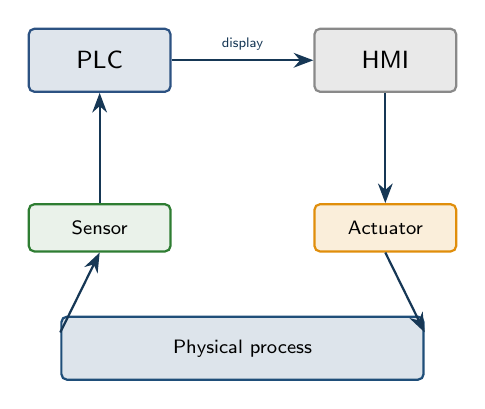
\begin{tikzpicture}[node distance=10mm]
  % Cyber row (top): PLC reads sensor, sends decisions to HMI for display
  \node[plc, minimum width=18mm] (plc) {PLC};
  \node[server, right=18mm of plc, minimum width=18mm] (srv) {HMI};
  % Physical row (bottom): sensor measures, actuator changes the process
  \node[sensor, below=14mm of plc, minimum width=18mm] (sens) {Sensor};
  \node[actuator, below=14mm of srv, minimum width=18mm] (act) {Actuator};
  \node[process, below=8mm of sens.south -| {$(sens)!0.5!(act)$}, minimum width=46mm, font=\scriptsize] (proc) {Physical process};
  % Vertical flows (no crossings)
  \draw[flow] (sens.north) -- (plc.south);
  \draw[flow] (srv.south) -- (act.north);
  % Horizontal cyber link
  \draw[flow] (plc.east) -- node[above, font=\tiny]{display} (srv.west);
  % Physical process at the bottom -- arrows enter the process from the sides
  \draw[flow] (act.south) -- ([yshift=2mm]proc.east) ;
  \draw[flow] ([yshift=2mm]proc.west) -- (sens.south);
\end{tikzpicture}
\end{columns}
\end{frame}

\begin{frame}{IT vs.\ OT --- Two Different Worlds}
\centering
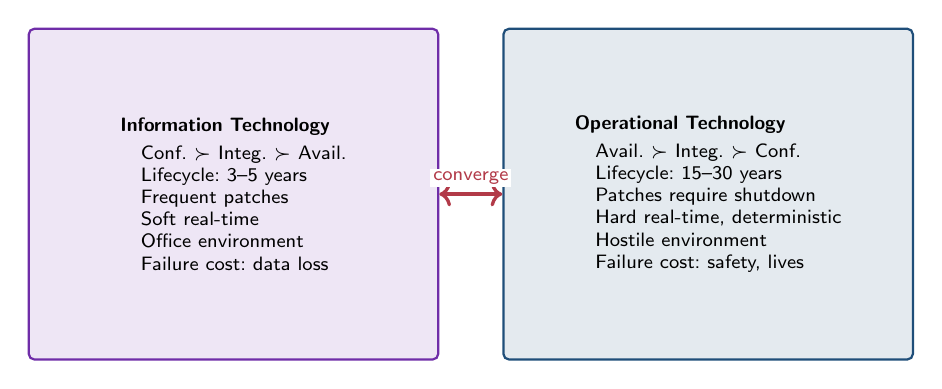
\begin{tikzpicture}[node distance=10mm]
  \node[isbox, fill=isIT!12, draw=isIT, minimum width=52mm, minimum height=42mm, align=left, font=\scriptsize] (it)
   {\textbf{Information Technology}\\[2pt]
     \quad Conf.\ $\succ$ Integ.\ $\succ$ Avail.\\
     \quad Lifecycle: 3--5 years\\
     \quad Frequent patches\\
     \quad Soft real-time\\
     \quad Office environment\\
     \quad Failure cost: data loss};
  \node[isbox, fill=isOT!12, draw=isOT, right=8mm of it, minimum width=52mm, minimum height=42mm, align=left, font=\scriptsize] (ot)
   {\textbf{Operational Technology}\\[2pt]
     \quad Avail.\ $\succ$ Integ.\ $\succ$ Conf.\\
     \quad Lifecycle: 15--30 years\\
     \quad Patches require shutdown\\
     \quad Hard real-time, deterministic\\
     \quad Hostile environment\\
     \quad Failure cost: safety, lives};
  \draw[<->, very thick, isAttack] (it.east) -- (ot.west) node[midway, above=2pt, font=\scriptsize, fill=white, inner sep=1pt] {converge};
\end{tikzpicture}
\end{frame}

\begin{frame}{The CIA Triad --- Inverted for OT}
\centering
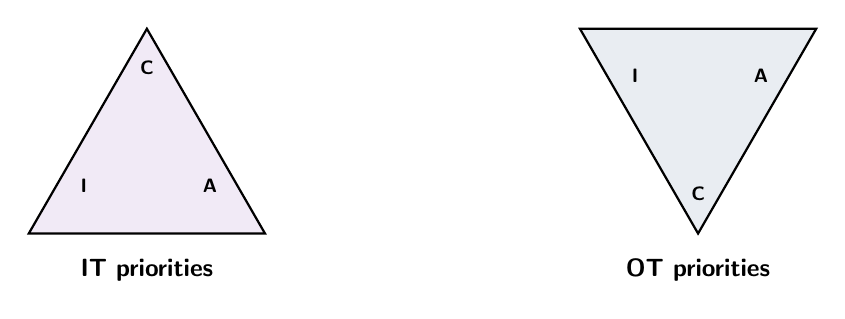
\begin{tikzpicture}
  % IT triangle
  \begin{scope}[shift={(-3.5,0)}]
    \draw[thick, fill=isIT!10] (0,0) -- (3,0) -- (1.5,2.6) -- cycle;
    \node[font=\scriptsize\bfseries] at (1.5, 2.1) {C};
    \node[font=\scriptsize\bfseries] at (0.7, 0.6) {I};
    \node[font=\scriptsize\bfseries] at (2.3, 0.6) {A};
    \node[font=\small\bfseries, below=2mm of {(1.5,0)}] {IT priorities};
  \end{scope}
  % OT triangle (flipped)
  \begin{scope}[shift={(3.5,0)}]
    \draw[thick, fill=isOT!10] (0,2.6) -- (3,2.6) -- (1.5,0) -- cycle;
    \node[font=\scriptsize\bfseries] at (1.5, 0.5) {C};
    \node[font=\scriptsize\bfseries] at (0.7, 2.0) {I};
    \node[font=\scriptsize\bfseries] at (2.3, 2.0) {A};
    \node[font=\small\bfseries, below=2mm of {(1.5,0)}] {OT priorities};
  \end{scope}
\end{tikzpicture}
\vspace{2mm}\par
\begin{importantbox}{Remember}
In OT, \textbf{availability} and \textbf{safety} dominate the CIA triad. A blocked alarm can blind an operator to a runaway reactor.
\end{importantbox}
\end{frame}

% --------------------------------------------------------------
\section{Context and History}

\begin{frame}{A Brief History of Industrial Control}
\centering
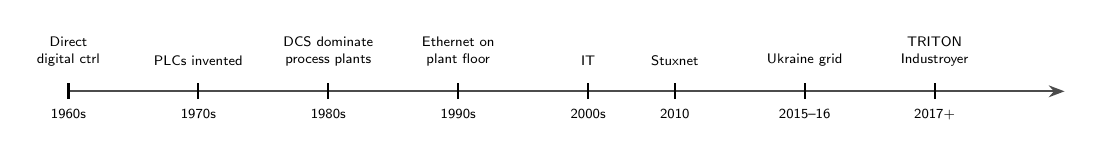
\begin{tikzpicture}[x=1.1cm]
  \draw[axisline] (0,0) -- (11.5,0);
  \foreach \x/\year/\label in {
    0/1960s/Direct\\digital ctrl,
    1.5/1970s/PLCs invented,
    3/1980s/DCS dominate\\process plants,
    4.5/1990s/Ethernet on\\plant floor,
    6/2000s/IT/OT\\convergence,
    7/2010/Stuxnet,
    8.5/2015--16/Ukraine grid,
    10/2017+/TRITON\\Industroyer}{
    \draw[thick] (\x,-1mm) -- (\x,1mm);
    \node[font=\tiny, below=1mm] at (\x,0) {\year};
    \node[font=\tiny, above=2mm, align=center] at (\x,0) {\label};
  }
\end{tikzpicture}
\vspace{2mm}\par
\small Each milestone made systems more capable -- and more reachable.
\end{frame}

\begin{frame}{Why Industrial Security Now?}
\centering
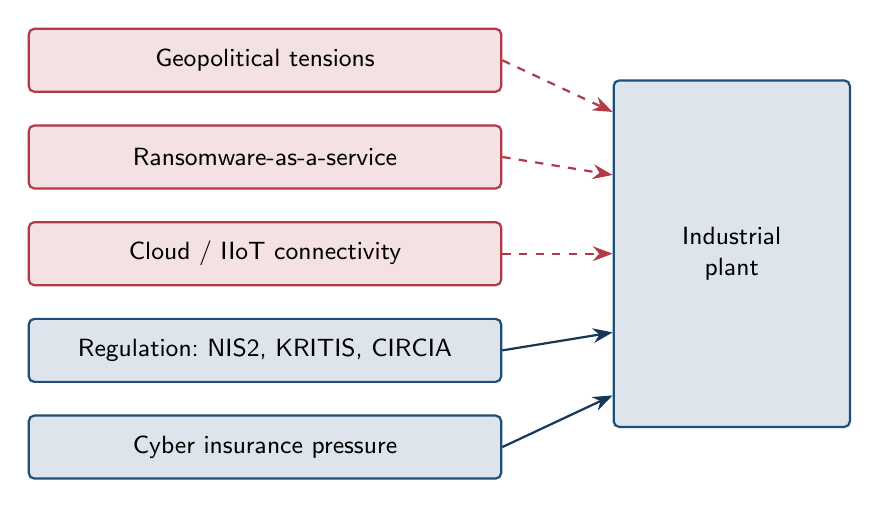
\begin{tikzpicture}[node distance=4mm]
  \node[isbox, fill=isAttack!15, draw=isAttack, minimum width=60mm] (a) {Geopolitical tensions};
  \node[isbox, fill=isAttack!15, draw=isAttack, minimum width=60mm, below=of a] (b) {Ransomware-as-a-service};
  \node[isbox, fill=isAttack!15, draw=isAttack, minimum width=60mm, below=of b] (c) {Cloud / IIoT connectivity};
  \node[isbox, fill=isOT!15, draw=isOT, minimum width=60mm, below=of c] (d) {Regulation: NIS2, KRITIS, CIRCIA};
  \node[isbox, fill=isOT!15, draw=isOT, minimum width=60mm, below=of d] (e) {Cyber insurance pressure};
  \node[process, right=14mm of c, minimum width=30mm, minimum height=44mm] (target) {Industrial\\plant};
  \draw[attack] (a.east) -- ([yshift=18mm]target.west);
  \draw[attack] (b.east) -- ([yshift=10mm]target.west);
  \draw[attack] (c.east) -- (target.west);
  \draw[flow]   (d.east) -- ([yshift=-10mm]target.west);
  \draw[flow]   (e.east) -- ([yshift=-18mm]target.west);
\end{tikzpicture}
\end{frame}

\begin{frame}{Stakeholders}
\centering
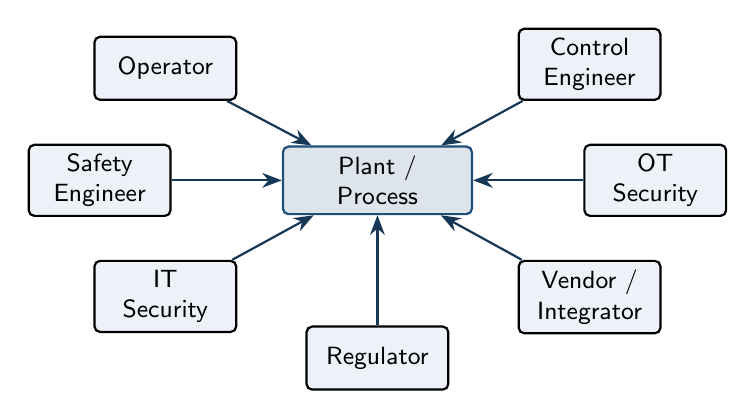
\begin{tikzpicture}[node distance=8mm]
  \node[process] (plant) {Plant /\\Process};
  \node[isbox, above left=of plant] (op) {Operator};
  \node[isbox, above right=of plant] (ce) {Control\\Engineer};
  \node[isbox, left=14mm of plant] (sa) {Safety\\Engineer};
  \node[isbox, right=14mm of plant] (sec) {OT\\Security};
  \node[isbox, below left=of plant] (it) {IT\\Security};
  \node[isbox, below right=of plant] (vend) {Vendor /\\Integrator};
  \node[isbox, below=14mm of plant] (reg) {Regulator};
  \foreach \n in {op,ce,sa,sec,it,vend,reg}{
    \draw[flow] (\n) -- (plant);
  }
\end{tikzpicture}
\vspace{2mm}\par
\small Industrial security is a team sport across roles that rarely sat together historically.
\end{frame}

% --------------------------------------------------------------
\section{Threat Setting and Misconceptions}

\begin{frame}{Common Misconceptions}
\centering
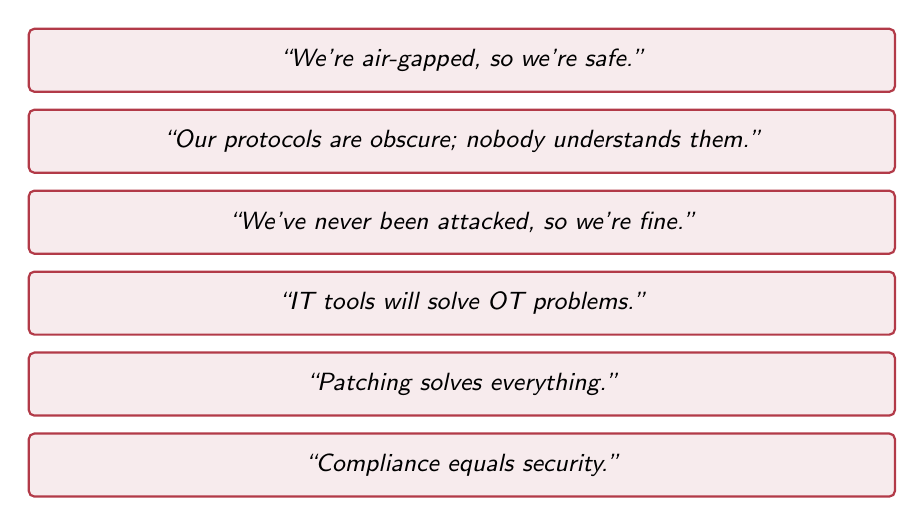
\begin{tikzpicture}[node distance=2mm]
  \node[isbox, fill=isAttack!10, draw=isAttack, minimum width=110mm, font=\small] (a)
    {\textit{``We're air-gapped, so we're safe.''}};
  \node[isbox, fill=isAttack!10, draw=isAttack, minimum width=110mm, font=\small, below=of a] (b)
    {\textit{``Our protocols are obscure; nobody understands them.''}};
  \node[isbox, fill=isAttack!10, draw=isAttack, minimum width=110mm, font=\small, below=of b] (c)
    {\textit{``We've never been attacked, so we're fine.''}};
  \node[isbox, fill=isAttack!10, draw=isAttack, minimum width=110mm, font=\small, below=of c] (d)
    {\textit{``IT tools will solve OT problems.''}};
  \node[isbox, fill=isAttack!10, draw=isAttack, minimum width=110mm, font=\small, below=of d] (e)
    {\textit{``Patching solves everything.''}};
  \node[isbox, fill=isAttack!10, draw=isAttack, minimum width=110mm, font=\small, below=of e] (f)
    {\textit{``Compliance equals security.''}};
\end{tikzpicture}
\end{frame}

\begin{frame}{Threat Pyramid -- Who Targets ICS?}
\centering
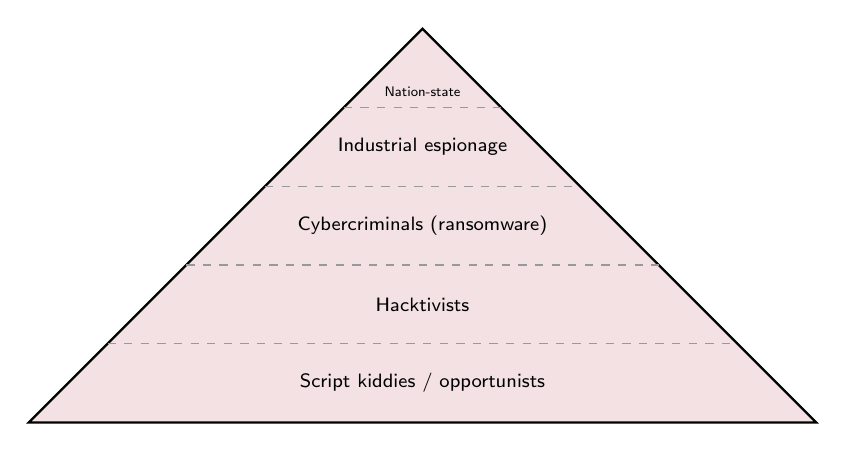
\begin{tikzpicture}
  % Pyramid outline (narrower base to keep labels clearly inside)
  \draw[thick, fill=isAttack!15] (0,0) -- (10,0) -- (5,5) -- cycle;
  % Tier dividers inside the pyramid (computed at heights 1..4)
  \foreach \y in {1,2,3,4}{
    \pgfmathsetmacro{\xl}{\y}
    \pgfmathsetmacro{\xr}{10-\y}
    \draw[dashed, black!40] (\xl,\y) -- (\xr,\y);
  }
  % Labels centred horizontally on the pyramid axis (x=5)
  \node[font=\scriptsize, align=center] at (5, 0.5) {Script kiddies / opportunists};
  \node[font=\scriptsize, align=center] at (5, 1.5) {Hacktivists};
  \node[font=\scriptsize, align=center] at (5, 2.5) {Cybercriminals (ransomware)};
  \node[font=\scriptsize, align=center] at (5, 3.5) {Industrial espionage};
  \node[font=\tiny, align=center] at (5, 4.2) {Nation-state};
\end{tikzpicture}
\vspace{2mm}\par
\small Capability rises as we move up; volume of actors falls.
\end{frame}

\begin{frame}{The Cost of ICS Incidents}
\centering
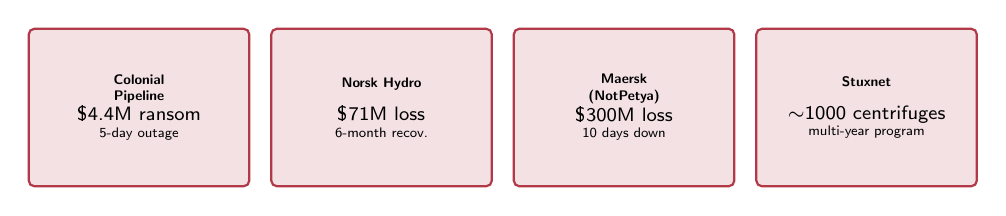
\begin{tikzpicture}[x=1.4cm]
  \node[isbox, fill=isAttack!15, draw=isAttack, font=\tiny, align=center, minimum width=28mm, minimum height=20mm] at (0,0) {\textbf{Colonial}\\\textbf{Pipeline}\\\scriptsize \$4.4M ransom\\5-day outage};
  \node[isbox, fill=isAttack!15, draw=isAttack, font=\tiny, align=center, minimum width=28mm, minimum height=20mm] at (2.2,0) {\textbf{Norsk Hydro}\\\\\scriptsize \$71M loss\\6-month recov.};
  \node[isbox, fill=isAttack!15, draw=isAttack, font=\tiny, align=center, minimum width=28mm, minimum height=20mm] at (4.4,0) {\textbf{Maersk}\\\textbf{(NotPetya)}\\\scriptsize \$300M loss\\10 days down};
  \node[isbox, fill=isAttack!15, draw=isAttack, font=\tiny, align=center, minimum width=28mm, minimum height=20mm] at (6.6,0) {\textbf{Stuxnet}\\\\\scriptsize $\sim$1000 centrifuges\\multi-year program};
\end{tikzpicture}
\vspace{2mm}
\begin{notebox}{Direct + indirect}
Recovery costs typically exceed ransom by 5--10$\times$. The lasting damage is reputation and regulatory.
\end{notebox}
\end{frame}

\begin{frame}{Industry 4.0 -- Convergence Pressure}
\centering
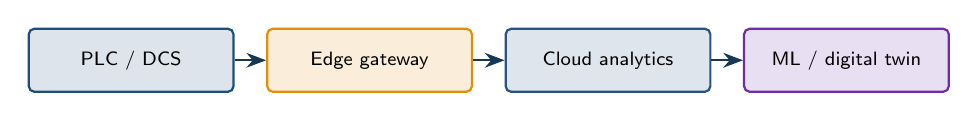
\begin{tikzpicture}[node distance=4mm]
  \node[isbox, fill=isOT!15, draw=isOT, minimum width=26mm, font=\scriptsize] (plc) {PLC / DCS};
  \node[isbox, fill=isAccent!15, draw=isAccent, right=of plc, minimum width=26mm, font=\scriptsize] (edge) {Edge gateway};
  \node[isbox, fill=isPLC!15, draw=isPLC, right=of edge, minimum width=26mm, font=\scriptsize] (cloud) {Cloud analytics};
  \node[isbox, fill=isIT!15, draw=isIT, right=of cloud, minimum width=26mm, font=\scriptsize] (ai) {ML / digital twin};
  \draw[flow] (plc) -- (edge); \draw[flow] (edge) -- (cloud); \draw[flow] (cloud) -- (ai);
\end{tikzpicture}
\vspace{2mm}
\begin{importantbox}{New attack surface}
Every cloud connector is a new ingress -- and a new authentication challenge for legacy field devices.
\end{importantbox}
\end{frame}

\begin{frame}{Career Paths in Industrial Security}
\begin{itemize}
  \item \textbf{OT Security Engineer} -- design, deploy, monitor controls; bridges IT and OT
  \item \textbf{Control Engineer with security focus} -- starts from process side
  \item \textbf{ICS Penetration Tester} -- offensive; specialised employers
  \item \textbf{Compliance / Audit} -- IEC 62443, NIS2 specialist
  \item \textbf{Incident Responder (OT)} -- on-call, often consulting-side (Dragos, Mandiant)
  \item \textbf{Researcher} -- vendor / academic; vulnerabilities, threat intel
\end{itemize}
\begin{tipbox}{Demand}
Headhunter reports consistently rank OT security in the top three hardest-to-fill cyber roles globally.
\end{tipbox}
\end{frame}

\begin{frame}{Section Roadmap}
\centering
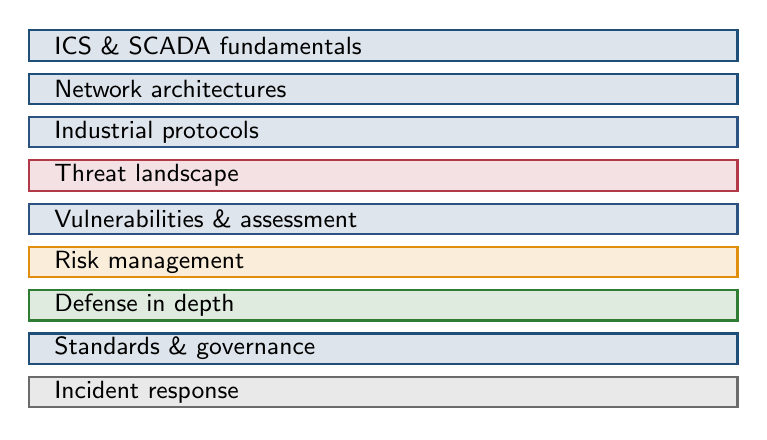
\begin{tikzpicture}[y=0.55cm, x=1cm]
  \foreach \i/\name/\col in {
    1/{ICS \& SCADA fundamentals}/isOT,
    2/{Network architectures}/isOT,
    3/{Industrial protocols}/isPLC,
    4/{Threat landscape}/isAttack,
    5/{Vulnerabilities \& assessment}/isPLC,
    6/{Risk management}/isAccent,
    7/{Defense in depth}/isNet,
    8/{Standards \& governance}/isOT,
    9/{Incident response}/isMute}{
    \draw[fill=\col!15, draw=\col, thick] (0,-\i) rectangle (9,-\i+0.7);
    \node[font=\small, anchor=west] at (0.2, -\i+0.35) {\name};
  }
\end{tikzpicture}
\end{frame}

\begin{frame}{Summary -- Section \sectionNumber}
\begin{takeawaybox}{Industrial security is different from IT security}
\begin{itemize}\setlength{\itemsep}{2pt}
  \item OT differs fundamentally from IT in goals, lifecycle, and tolerance for failure.
  \item Availability and safety dominate the CIA triad in industrial contexts.
  \item Adversaries today span from script kiddies to nation-state APTs.
  \item The next sections build the toolbox: components, networks, protocols, defenses.
\end{itemize}
\end{takeawaybox}
\end{frame}

\closingframe

\end{document}
